\section{INTRODUÇÃO}

O setor agropecuário brasileiro tem se destacado nas últimas décadas por seu crescimento proveniente da aplicação de novas tecnologias ao clima tropical e a incorporação de novas áreas de terras \cite{brasil19}. Segundo dados dos censos agropecuários, entre $2006$ e $2017$, tanto a área total quanto a produção agrícola e pecuária vivenciaram crescimento. Neste período houve um acréscimo de cerca de $5,8\%$ na área total dos estabelecimentos agropecuários \cite{ibge19}. Com relação à sua participação no PIB, em 2019, a parcela do agronegócio brasileiro foi de  $20,5\%$  do PIB nacional. Já em 2020, o setor agropecuário brasileiro alcançou a participação de $26,6\%$ do PIB. Em valores monetários, o PIB do País totalizou R\$ $7,45$ trilhões em 2020, e a participação do agronegócio chegou a quase R\$ $2$ trilhões \cite{cepea21}. 

Dada a relevância do setor agropecuário na economia brasileira, é necessário destacar que este ramo apresenta características muito específicas com relação à magnitude dos riscos aos quais está sujeito \cite{burgo05}. Alguns riscos mais relevantes se devem, principalmente, às instabilidades climáticas e ameaças sanitárias, que podem afetar a produção, ou à razões de mercado, como variações das taxas de câmbio e juros, ou a condições ligadas ao ambiente de negócios, tais como, alterações em marcos regulatórios e em políticas públicas. Todos esses fatores geram variações na renda do setor, que devem ser enfrentadas por meio de políticas de apoio à gestão de riscos \cite{brasil21}. 

Uma gestão de riscos apropriada tem potencial de afetar de forma positiva a estabilidade da renda do produtor e sua própria permanência no setor agropecuário. O gerenciamento de riscos agropecuários pode ocorrer de diversas maneiras, no entanto, a contratação de seguro é uma das medidas mais comuns. O seguro rural é uma importante ferramenta de mitigação de riscos e proteção da renda. Esta modalidade de seguro atua no sentido de amenizar as perdas e possibilitar a recuperação da capacidade financeira do produtor rural em caso de ocorrência de sinistros \cite{brasil19b}. 

Nesse sentido, o presente trabalho tem por objetivo, avaliar a distribuição espacial do seguro rural nos municípios brasileiros entre 2006 e 2019. Para tanto, busca-se investigar se, no Brasil, as variáveis de seguro rural se distribuem de forma aleatória no espaço ou se há padrões de distribuição espacial. Além disso, através da análise da distribuição espacial do seguro rural no período, busca-se identificar se há regiões que tiveram alterações significativas no número de contratações de seguro. Por fim, este estudo busca fornecer informações para o debate de aperfeiçoamentos no sistema de seguro rural brasileiro, de forma a contribuir para uma agricultura mais eficiente e com menores riscos para o produtor rural.

O trabalho está estruturado da seguinte forma: a próxima seção apresenta uma breve revisão de literatura sobre o seguro rural e a análise exploratória de dados espaciais. A terceira seção apresenta os dados, os procedimentos de análise e recursos computacionais que serão utilizados. A quarta seção apresenta resultados e discussões. A última seção apresenta as considerações finais.

%\newpage


\section{MATERIAL E MÉTODOS}\label{material_e_metodos}

%O objetivo dessa seção é apresentar os dados utilizados no trabalho, descrever a metodologia e os recursos computacionais utilizados na presente análise.

\subsection{DADOS}

% Fonte dos Dados 

Os dados de seguro rural utilizados neste trabalho foram obtidos no endereço eletrônico do Ministério da Agricultura, Pecuária e Abastecimento (MAPA) \cite{brasil21}. Foram utilizados dados com valores anuais a partir do ano de $2006$ até o ano de $2019$ (último ano disponível até então) para os dados municipais. Os dados agregados são provenientes do Atlas do Seguro Rural do MAPA e apresentam periodicidade anual a partir do ano de $2006$. Também foram utilizados dados que contém atributos geográficos, como a posição e o formato, do território brasileiro. Esses dados estão disponíveis no endereço eletrônico do Instituto Brasileiro de Geografia e Estatística \cite{ibge20}.

O conjunto de dados de seguro rural possui informação referente à localização geográfica da contratação do seguro rural. No entanto, foram detectadas algumas divergências relacionadas a distritos ou outras localidades, como fazendas e vilarejos, que foram apontados como o local referente à contratação do seguro. 

Para corrigir essas divergências, de forma a ter informações referentes apenas aos municípios brasileiros, as informações relacionadas às demais localidades foram acrescentadas aos municípios correspondentes. Para a identificação, foi feita uma busca de cada localidade que não tinha correspondência com os municípios brasileiros. Essa busca foi feita inicialmente no site \textit{google maps}, contendo, como termo de busca, o nome da localidade e o seu estado \footnote{Foi considerado que a informação referente aos Estados estava correta nos dados do MAPA}. Nos casos em que a informação do município ao qual a localidade pertencia estava disponível no resultado da pesquisa, o nome do município era utilizado em uma segunda busca no site \textit{Portal Cidades} do IBGE \footnote{\url{https://cidades.ibge.gov.br}}. O \textit{Portal Cidades} apresenta, na maioria dos casos, a divisão territorial e administrativa atualizada, de forma a possibilitar a correção das divergências nos dados. Nos casos em que a informação do município ao qual a localidade pertencia não estava disponível no resultado da pesquisa, o nome da localidade era utilizado como termo de busca de CEPs no site dos Correios \footnote{\url{https://buscacepinter.correios.com.br/app/localidade_logradouro/index.php}}. Para os casos em que não foi possível encontrar nenhum resultado com relação ao município correspondente, a localidade em divergência foi atribuída ao município geograficamente mais próximo. 

\subsection{ANÁLISE DOS DADOS} 

Após uma análise exploratória dos dados, foi realizada a primeira parte da Análise Exploratória de Dados Espaciais (AEDE), onde os dados agregados por municípios serão apresentados por meio de mapas temáticos, de forma a ilustrar o padrão espacial das variáveis de seguro rural. No segundo passo da AEDE, o valor do \textit{I} de Moram global foi calculado e sua significância obtida por meio do pseudo valor-$p$, obtido a partir de $999$ permutações aleatórias. Neste estudo, foi considerado um nível de significância $\alpha = 0,05$. Foi adotada a matriz de pesos espaciais de contiguidade com a convenção rainha, considerando os vizinhos de primeira ordem. Tal matriz foi adotada por ser a mais utilizada na literatura em trabalhos semelhantes. 

Para a construção da matriz de pesos espaciais, foram retirados os municípios de Fernando de Noronha, que se constitui em um arquipélago pertencente ao estado de Pernambuco, e Ilhabela, arquipélago no litoral norte do estado de São Paulo. Estes municípios foram desconsiderados pois, além de se constituírem de ilhas, não possuem nenhuma apólice de seguro rural contratada durante os anos em análise. Uma vez definida a matriz, se o valor do \textit{I} de Moran global for significativo, a hipótese de aleatoriedade espacial deve ser rejeitada e há evidências de que há uma autocorrelação positiva. 

O terceiro passo da análise espacial das variáveis de seguro rural consistiu na obtenção dos mapas \textit{LISA}, de forma a identificar padrões locais de autocorrelação espacial e \textit{outliers} espaciais. Esses mapas ilustram cada uma das observações e indicam se seus valores foram considerados significativos em relação à estatística do I de Moran local. 
% Discussão sobre o tipo de matriz de ponderação utilizada

\subsection{RECURSOS COMPUTACIONAIS}  
% Linguagem de programação 
Esse estudo foi feito utilizando a linguagem de programação \textit{Python} \cite{python17}, através da interface \textit{Jupyter} \cite{jupyter17} \cite{perez07} \cite{kluyver19};
Além disso, foram utilizadas as seguintes bibliotecas: 
\textit{Pandas} \cite{mckinney10}, que é uma ferramenta  para análise e manipulação de dados;
\textit{NumPy} \cite{walt11}, que é destinado a possibilitar a computação numérica com \textit{Python};
\textit{SciPy} (JONES et al., 2001); % rever essa citação
\textit{Matplotlib} \cite{hunter07} e \textit{Seaborn} \cite{waskom14}, que são bibliotecas para criar visualizações  de dados em \textit{Python};
\textit{jenkspy} para a utilização do algoritmo Fisher Jenks \cite{jenks77};
\textit{Geopandas} \cite{jordahl14} e \textit{PySAL} \cite{rey07} que possibilitam a análise espacial.


%\newpage
\section{RESULTADOS E DISCUSSÃO}

\subsection{O SEGURO RURAL NO BRASIL} 

Inicialmente, serão apresentados dados ilustrativos da trajetória do Seguro Rural no Brasil. Serão analisados dados anuais referentes ao número de apólices contratadas, ao número de apólices indenizadas, aos valores de subvenção, indenização e prêmio. Também serão apresentados dados referentes à participação das seguradoras e das principais culturas no número de apólices contratadas. Foram utilizados dados da Plataforma Atlas do Seguro Rural. É importante destacar que os valores referentes ao ano de $2021$ ainda não estavam consolidados na data do presente estudo.

\subsubsection{Apólices contratadas}

Nesta seção, serão analisados dados anuais referentes às apólices de seguro rural contratadas e os respectivos valores de prêmio e subvenção. 

No gráfico da Figura \ref{apolices_produtores} é possível observar a evolução do número de produtores e do número de apólices de seguro rural contratadas no período de $2006$ a $2020$. Durante o período analisado, cada produtor contratou, em média, $1,48$ apólices de seguro rural. O número de apólices contratadas tem um crescimento de cerca de $8,69$ vezes durante o período. Entre os anos $2014$ e $2015$, ocorre uma queda de $66,08\%$ nas apólices contratadas. Por sua vez, o número de produtores cresceu $6,36$ vezes entre $2006$ e $2020$.

\begin{figure}[H]
	\centering
	\caption{Número de produtores e apólices de seguro rural contratadas. Brasil $2006 - 2020$}
	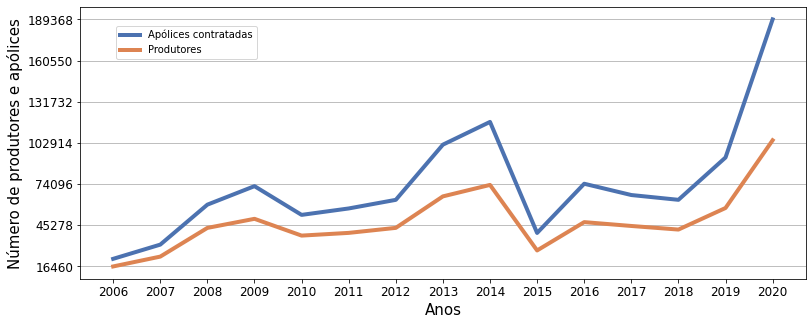
\includegraphics[width=0.8\textwidth]{figuras/apolices_produtores.png}\\
	\small \textsuperscript {Fonte: Elaboração própria a partir de dados da Plataforma Atlas do Seguro Rural (Mapa, 2021).}
    \label{apolices_produtores}
\end{figure}

É importante destacar que, no ano de $2021$, até o mês de junho, haviam $66.928$ apólices contratadas \cite{brasil21}. Apesar do valor ser baixo se comparado ao ano de $2020$ ($189.368$ apólices), já é superior a $56,25\%$ dos anos anteriores. Padrão semelhante se observa com o número de produtores. No ano de $2021$, até o mês de junho haviam sido contabilizados $47.472$ produtores segurados.

\subsubsection{Valores do prêmio e de subvenção ao prêmio de seguro rural}

O gráfico da Figura \ref{soma_ano_values} apresenta a evolução dos valores em milhões de reais de subvenção ao prêmio de seguro rural, prêmio pago pelo produtor e prêmio recebido pela seguradora entre $2006$ a $2020$. Observa-se que, com exceção do ano de $2014$, é possível notar uma tendência de crescimento dos valores de subvenção e prêmio pagos no período analisado. No ano de 2014, devido à contenções, o governo federal liberou apenas R\$ $400$ milhões dos R\$ $700$ milhões previstos para subsidiar o seguro rural. Esta contenção dos gastos governamentais pode ser um fator a ser considerado na queda dos valores do seguro rural ocorrida entre os anos de $2014$ e $2015$ \cite{andrade21}.

\begin{figure}[H]
	\centering
	\caption{Valores do prêmio e de subvenção ao prêmio de seguro rural. Brasil $2006 - 2020$}
	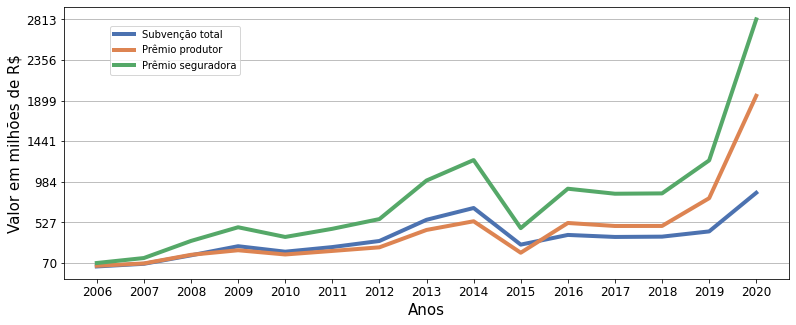
\includegraphics[width=0.8\textwidth]{figuras/soma_ano_values.png}\\
	\small \textsuperscript {Fonte: Elaboração própria a partir de dados da Plataforma Atlas do Seguro Rural (Mapa, 2021).}
    \label{soma_ano_values}
\end{figure}

Em $2021$, até o mês de junho, o valor do prêmio pago à seguradora já havia alcançado R\$$1,25$ bilhões, o quarto maior valor registrado e cerca de $50.59\%$ maior que a média (Mapa, 2021). O prêmio do produtor referente ao período de janeiro a junho de $2021$ já era equivalente à R$\$0,77$ bilhões, valor cerca de $69,67\%$ maior que a média do prêmio de responsabilidade do produtor. O valor concedido na forma de subvenção ao prêmio em $2021$ também é o quarto maior valor registrado, cerca de $25,96\%$ maior que a média do valores de subvenção concedidos. Além disso, a partir do ano de $2016$, a parcela do prêmio sob responsabilidade do produtor passa a superar a parcela concedida pelo governo na forma de subvenção.

Os valores da soma da importância segurada em milhões de reais são apresentados no gráfico da Figura \ref{total_segurado_mil}. Observa-se que há crescimento dos valores segurados, com destaque para o crescimento entre os anos de $2019$ e $2020$, em que o os valores mais que duplicaram. Considerando o período entre $2006$ e $2020$, o crescimento da importância segurada foi de $15,55$ vezes o valor de $2006$. Também é possível observar que, entre os anos de $2014$ e $2015$, ocorreu uma queda de $70,68\%$ do valor segurado.  

Em $2020$, o Programa de Subvenção ao Prêmio do Seguro Rural aplicou R\$ $880$ milhões, ou seja, o dobro do valor executado no ano de  $2019$. Para o ano de $2021$, a estimativa apresentada pelo Ministério da Agricultura e Abastecimento foi um aumento de R\$ $1$ bilhão a verba destinada ao PSR (Mapa, 2021).

\begin{figure}[H]
	\centering
	\caption{Soma da importância segurada (R\$ milhões). Brasil $2006 - 2020$}
	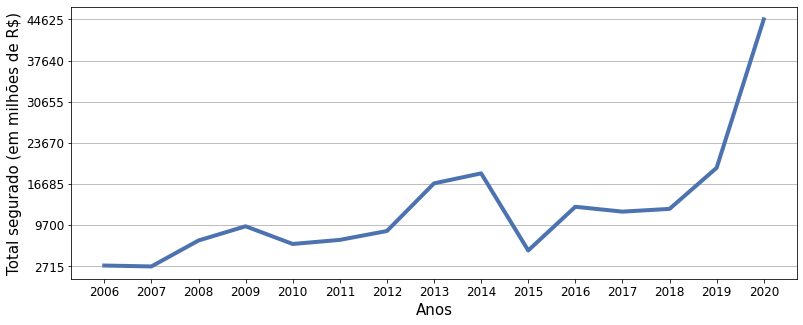
\includegraphics[width=0.8\textwidth]{figuras/total_segurado_mil.png}\\
	\small \textsuperscript {Fonte: Elaboração própria a partir de dados da Plataforma Atlas do Seguro Rural (Mapa, 2021).}
    \label{total_segurado_mil}
\end{figure}

No ano de $2014$, o total segurado chegou a R$\$18.462,88$ milhões, no entanto, em $2015$ a soma da importância caiu para R$\$5.398,54$ milhões, o terceiro valor mais baixo do período. O valor mais alto ocorre no ano de $2020$ em que o valor segurado foi de R$\$45,7$ bilhões, o maior desde o início do programa em $2005$.

O valor da importância segurada alcançou $R\$14.4$ bilhões até o mês de junho de $2021$. Este valor é o quinto maior valor da série e já é maior que $25\%$ dos valores registrados nos anos anteriores 

\subsubsection{Área segurada em hectares}

A Figura \ref{area_segurada} apresenta o total da área segurada em hectares nos municípios do Brasil entre os anos de  $2006$ e  $2020$. É possível observar que, a área agrícola segurada (Figura \ref{area_segurada}) no país praticamente dobrou entre $2019$ e $2020$, quando alcança o maior valor, $13,7$ milhões de hectares, o que representa $20\%$ da área total agrícola do país. O aumento de área em relação a $2019$ é de $98\%$. O maior valor registrado em anos anteriores foi em $2014$, quando foram segurados $9,4$ milhões de hectares. 

\begin{figure}[H]
	\centering
	\caption{Total da área segurada em hectares. Brasil $2006 - 2020$}
	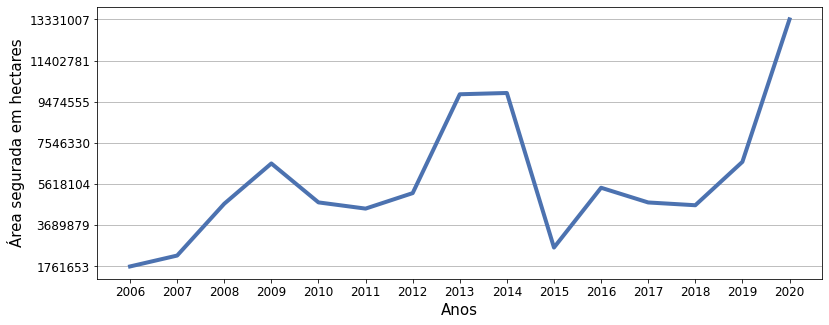
\includegraphics[width=0.8\textwidth]{figuras/area_segurada.png}\\
	\small \textsuperscript {Fonte: Elaboração própria a partir de dados do Ministério da Agricultura, Pecuária e Abastecimento (MAPA).}
    \label{area_segurada}
\end{figure}

No ano de $2021$, até o mês de junho, foram segurados cerca de $3.76$ milhões de hectares. Esse valor representa cerca de $71.76\%$ da área segurada em $2020$ (Mapa, 2021). 

\subsubsection{Indenizações}

Com relação ao número de indenizações,  o gráfico da Figura \ref{apolices_indenizadas} apresenta a evolução das apólices indenizadas ao longo do período analisado. O menor número de indenizações é $389$ em $2006$ e o maior valor ocorreu no ano de $2018$, sendo igual a $17.625$ indenizações. Durante o período, ocorre em média um número de $8.110$ apólices indenizadas por ano, sendo que o crescimento no número de apólices indenizadas entre $2006$ e $2019$ foi de $2230,59\%$. 

\begin{figure}[H]
	\centering
	\caption{Número de apólices de seguro rural indenizadas. Brasil $2006 - 2019$}
	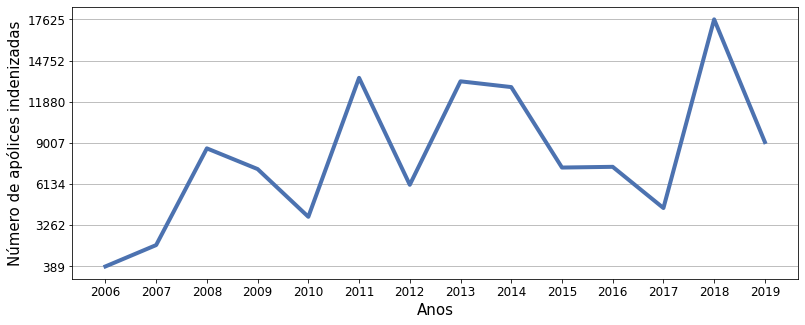
\includegraphics[width=0.8\textwidth]{figuras/apolices_indenizadas.png}\\
	\small \textsuperscript {Fonte: Elaboração própria a partir de dados do Ministério da Agricultura, Pecuária e Abastecimento (MAPA)}
    \label{apolices_indenizadas}
\end{figure}

Os valores pagos como indenização entre os anos de $2006$ e $2019$ são apresentados no gráfico da Figura \ref{valor_indenizacoes} e variam entre R\$ $20.699.785,74$ em $2006$ e R\$ $924.988.210,45$ em $2018$. A média do valor das indenizações foi de R\$ $345.525.736,50$ no período analisado. 

\begin{figure}[H]
	\centering
	\caption{Valor das indenizações de seguro rural pagas (R\$ milhões). Brasil $2006 - 2019$}
	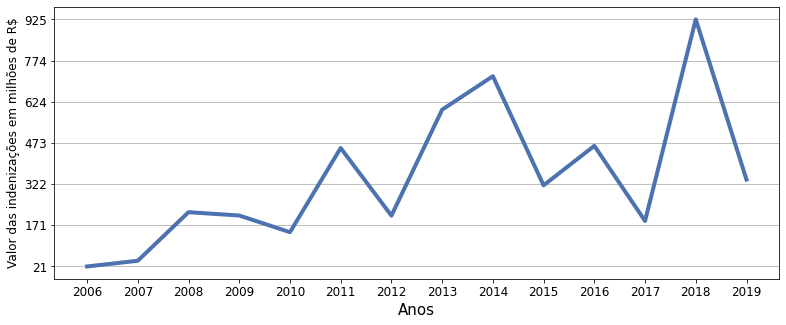
\includegraphics[width=0.8\textwidth]{figuras/valor_indenizacoes.png}\\
	\small \textsuperscript {Fonte: Elaboração própria a partir de dados do Ministério da Agricultura, Pecuária e Abastecimento (MAPA)}
    \label{valor_indenizacoes}
\end{figure}

\subsubsection{Taxa média de contratação de seguro rural}

O gráfico apresentado na Figura \ref{taxa_media} mostra a trajetória da taxa de contratação do seguro rural. É possível constatar que a taxa se eleva, em média, de $4,7\%$ em $2006$ para $ 7,46\%$ em $2020$. Até o mês de junho de $2021$ o valor da taxa média havia alcançado $9,79\%$, o segundo maior valor da série, sendo superado pela taxa média cobrada em $2015$, que foi de $10,3\%$.  

\begin{figure}[H]
	\centering
	\caption{Taxa média anual de contratação do prêmio ao seguro rural. Brasil $2006 - 2020$}
	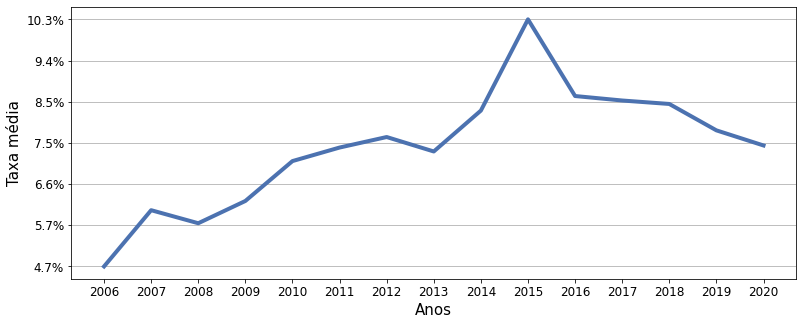
\includegraphics[width=0.8\textwidth]{figuras/taxa_media.png}\\
	\small \textsuperscript {Fonte: Elaboração própria a partir de dados da Plataforma Atlas do Seguro Rural (Mapa, 2021).}
   \label{taxa_media}
\end{figure}

Segundo Santos e Silva (2017), espera-se que, à medida que o sistema de seguro rural se consolida, reduzam-se os preços das apólices devido aos ganhos de produtividade agropecuária e da redução de fatores de risco. Essas reduções podem ocorrer devido à adoção das orientações do zoneamento agrícola, de um maior conhecimento do histórico de eventos climáticos e dos sinistros ocorridos e, até mesmo em função da adoção de tecnologias, como o uso de irrigação etc. No entanto, essa redução das taxas não ocorreu no período analisado, como observado na Figura \ref{taxa_media}. 

\subsubsection{Culturas}

A Figura \ref{percent_cult_apol} apresenta o percentual da participação das maiores culturas no número de apólices de seguro rural contratadas. A análise desse gráfico permite identificar que, com exceção de $2015$, a cultura da soja foi a que mais contratou seguro rural. Além disso, observa-se que o milho 2ª safra \footnote{Nesse caso o milho de 2ª safra é listado em separado devido aos distintos graus de risco em relação à 1ª safra \cite{santos17}.} tem cada vez mais aumentado sua participação no número de apólices contratadas. O milho 1ª safra, por sua vez, tem participação que varia entre $1,23\%$ e $16,46\%$, com média de  $6,16\%$ ao longo do período. A participação da cultura da maçã na contratação de seguro rural permanece relativamente estável ao longo do período, variando entre $8,79\%$ e $14,72\%$. 

\begin{figure}[H]
	\centering
	\caption{Percentual da participação das maiores culturas no número de apólices de seguro rural contratadas. Brasil $2006 - 2019$}
    	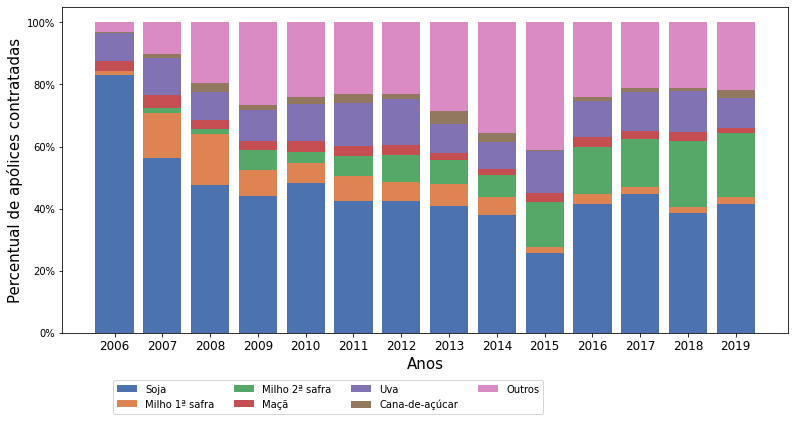
\includegraphics[width=0.8\textwidth]{figuras/percent_apolic_cult.png}\\
	\small \textsuperscript {Fonte: Elaboração própria a partir de dados do Ministério da Agricultura, Pecuária e Abastecimento (MAPA)}
    \label{percent_cult_apol}
\end{figure}

A Tabela\ref{percent_culturas} apresenta a participação percentual de grupos de culturas em variáveis do seguro rural. É possível constatar que entre os anos de $2006$ e $2020$ as culturas de grãos foram responsáveis por $74,85\%$ das apólices contratadas, seguida das culturas de frutas com $14,74\%$ das apólices no período. Em terceiro lugar está a cultura de olerícolas, com cerca de $3,36\%$ de participação na contratação de apólices de seguro rural. Uma estrutura semelhante de participação percentual de grupos de culturas pode ser observada com relação à participação no valor total segurado. O grupo de cultura que mais se destaca é a dos grãos, com $74,88\%$ do total segurado, seguido das frutas e do café, com $9,55\%$ e $4,04\%$, respectivamente. 

\begin{small}
\begin{table}[H]
\caption{Participação percentual das culturas nos valores do seguro rural. Brasil $2006-2020$}\label{percent_culturas}
 \footnotesize
\vspace{0.05cm}
\begin{tabularx}{\textwidth}{lRRRRR}
    \hline \\[-1.9ex]	 
    Cultura    & \% das apólices & \% do total segurado & \% do premio total & \% de subvenção & Taxa média \\
    \hline \\[-1.9ex]	 
    Grãos      & 74,85\%         & 74,88\%              & 78,86\%            & 77,35\%         & 7,70\%     \\
    Frutas     & 14,74\%         & 9,55\%               & 13,14\%            & 16,07\%         & 9,17\%     \\
    Olerícolas & 3,36\%          & 2,74\%               & 3,17\%             & 2,85\%          & 7,64\%     \\
    Café       & 3,07\%          & 4,04\%               & 2,19\%             & 1,61\%          & 3,15\%     \\
    Cana       & 2,08\%          & 2,98\%               & 0,77\%             & 0,69\%          & 1,63\%     \\
    Pecuária   & 0,73\%          & 1,16\%               & 0,77\%             & 0,32\%          & 3,26\%     \\
    Floresta   & 0,30\%          & 3,51\%               & 0,42\%             & 0,35\%          & 1,60\%     \\
    Outros     & 0,88\%          & 1,13\%               & 0,68\%             & 0,75\%          & 4,64\%     \\ 
    \hline 
\end{tabularx}
%\vspace{0.5cm}
\small \textsuperscript{Fonte: Elaboração própria a partir de dados da Plataforma Atlas do Seguro Rural (Mapa, 2021).  }\\
\end{table}
\end{small}

Além disso, é possível observar na Tabela\ref{percent_culturas}, os percentuais de subvenção ao prêmio de seguro rural e os valores da taxa média de contratação do seguro. As taxas cobradas durante o período para a cultura de grãos foi de $7,70\%$, a taxa cobrada das culturas de frutas foi de $9,17\%$ e, as olerícolas tiveram uma taxa média de contratação de $7,64\%$. Os percentuais de subvenção dessas culturas são, também, os mais altos: $77,35\%$ de subvenção para os grãos, $16,07\%$ para as culturas de frutas e $2,85\%$ para as olerícolas. Ou seja, os grupos de culturas com maior demanda pelo seguro, além de apresentarem os maiores valores de apólices e a maior quantidade e valores de sinistros, são também aqueles com maiores taxas médias. 
De acordo com  Santos e Silva (2017), este fato pode apontar para a possibilidade de dois fenômenos a serem melhor examinados. O primeiro diz respeito à situação em que as maiores taxas resultam do fato de que maiores subvenções são dadas a cultivos de maior risco. O segundo fenômeno possível é que as taxas sejam mais altas, principalmente no caso dos produtores que adotam o ZARC, com elevada tecnologia produtiva, alta produtividade e não têm estas características levadas em consideração como informação que contribui para a redução das taxas. Dessa forma, se por um lado o seguro agrícola não se consolida sem a subvenção dada pelo Estado, por outro, é possível que esse sistema de subvenção ao prêmio crie distorções no mercado de seguro rural. 

\subsubsection{Seguradoras}

A Tabela\ref{seguradoras} exibe a distribuição das fatias de mercado das seguradoras, entre $2006$ e $2020$. Apesar de, as seguradoras passaram de cinco, em $2006$, para $16$ companhias aptas a operar com seguro rural em $2020$, é possível constatar que há uma concentração do mercado de seguro em um número reduzido de seguradoras. 

\begin{small}
\begin{table}[H]
\caption{Participação de mercado das seguradoras. Brasil $2006-2020$}\label{seguradoras}
 \footnotesize
\vspace{0.05cm}
\begin{tabularx}{\textwidth}{lRRRRRRR}
    \hline \\[-1.9ex]	 
    Seguradora         & Apólices        & \% do número de apólices  & Beneficiários  & \% dos beneficiários  & Área segurada (em mil ha)  & \% de área segurada   \\
    \hline \\[-1.9ex]	 
    Brasilseg         &  $410.892$      &  $37,23  $                &  $95.769$                    &  $26,85  $            &  $48.076,26$       & $55,31  $              \\
    Mapfre            &  $149.389$      &  $13,54  $                &  $49.274$                    &  $13,82  $            &  $7.309,17$        &  $8,41  $               \\
    Essor             &  $119.087$      &  $10,79  $                &  $38.995$                    &  $10,93  $            &  $4.603,47$        &  $5,30  $               \\
    Swiss Re          &  $91.410$       &  $8,28  $                 &  $34.483$                    &  $9,67  $             &  $7.870,31$        &  $9,06  $               \\
    Nobre             &  $82.500$       &  $7,48  $                 &  $29.053$                    &  $8,15  $             &  $2.747,88$        &  $3,16  $               \\
    Allianz           &  $66.983$       &  $6,07  $                 &  $21.210$                    &  $5,95  $             &  $5.387,98$        &  $6,20  $               \\
    Sancor            &  $49.567$       &  $4,49  $                 &  $22.516$                    &  $6,31  $             &  $3.210,37$        &  $3,69  $               \\
    Fairfax           &  $35.343$       &  $3,20  $                 &  $18.349$                    &  $5,14  $             &  $2.055,87$        &  $2,37  $               \\
    Porto Seguro      &  $26.306$       &  $2,38  $                 &  $6.152$                     &  $1,72  $             &  $259,33$          &  $0,30  $               \\
    Newe              &  $22.741$       &  $2,06  $                 &  $12.337$                    &  $3,46  $             &  $1.469,10$        &  $1,69  $               \\
    Tokio Marine      &  $19.808$       &  $1,79  $                 &  $11.263$                    &  $3,16  $             &  $1.722,64$        &  $1,98  $               \\
    Too               &  $14.844$       &  $1,35  $                 &  $9.768$                     &  $2,74  $             &  $1.163,48$        &  $1,34  $               \\
    Aliança do Brasil &  $7.200$        &  $0,65  $                 &  $3.294$                     &  $0,92  $             &  $593,19$          &  $0,68  $               \\
    Excelsior         &  $4.472$        &  $0,41  $                 &  $2.292$                     &  $0,64  $             &  $238,97$          &  $0,27  $               \\
    Sompo             &  $3.062$        &  $0,28  $                 &  $1.901$                     &  $0,53  $             &  $181,66$          &  $0,21  $               \\
    Itaú              &  $9$            &  $0,00  $                 &  $9$                         &  $0,00  $             &  $25,10$           &  $0,03  $               \\
    \hline \\[-1.9ex]
    \textbf{Total}    & \textbf{1.103.613} & \textbf{100  }         & \textbf{213.692}             & \textbf{100  }        & \textbf{86.914,79} & \textbf{100  }\\
	\hline 
\end{tabularx}
%\vspace{0.5cm}
\small \textsuperscript{Fonte: Elaboração própria a partir de dados da Plataforma Atlas do Seguro Rural (Mapa, 2021).}\\
\footnotesize{Nota: Valores acumulados $2006 -- 2020$}\\
\end{table}
\end{small}

Ao se analisar a participação no percentual do número de apólices de seguro rural, percebe-se que apenas as três maiores seguradoras (Brasilseg, Mapfre e Essor) concentram cerca de $61,56\%$ do mercado. Com relação ao percentual dos beneficiários, as três maiores seguradoras contam com cerca de $51,60\%$ dos beneficiários durante o período analisado. A concentração é ainda maior quando se analisa o percentual da área segurada, sendo que a  maior seguradora do ramo (Brasilseg) conta com um percentual de $55,31\%$ da área segurada em hectares. As três maiores seguradoras são responsáveis pelo seguro de $72,78\%$ da área segurada. 

A próxima seção tem como objetivo apresentar os resultados da análise da distribuição espacial dos dados do seguro rural no Brasil. 

\subsection{DISTRIBUIÇÃO ESPACIAL}

A análise da distribuição espacial das variáveis se inicia com a visualização dos mapas temáticos. Por meio destes mapas, busca-se identificar visualmente se há a ocorrência de padrões na distribuição espacial das variáveis do seguro rural.

O primeiro grupo de mapas, apresentado na Figura \ref{map_apolices}, exibe a distribuição espacial do número de apólices contratadas nos municípios brasileiros entre os anos de 2006 e 2019. Para a construção dos mapas, os valores da variável foram divididos em 5 intervalos \footnote{Para a criação dos intervalos foi aplicado algoritmo Fisher Jenks aos valores das variáveis diferentes de $0$ e os intervalos foram criados tendo como referência os valores do ano de 2019 \cite{jenks77}}.

\begin{figure}[H]
	\centering
	\caption{Total segurado por municípios brasileiros, de 2006 a 2019 (em mil R\$)}
	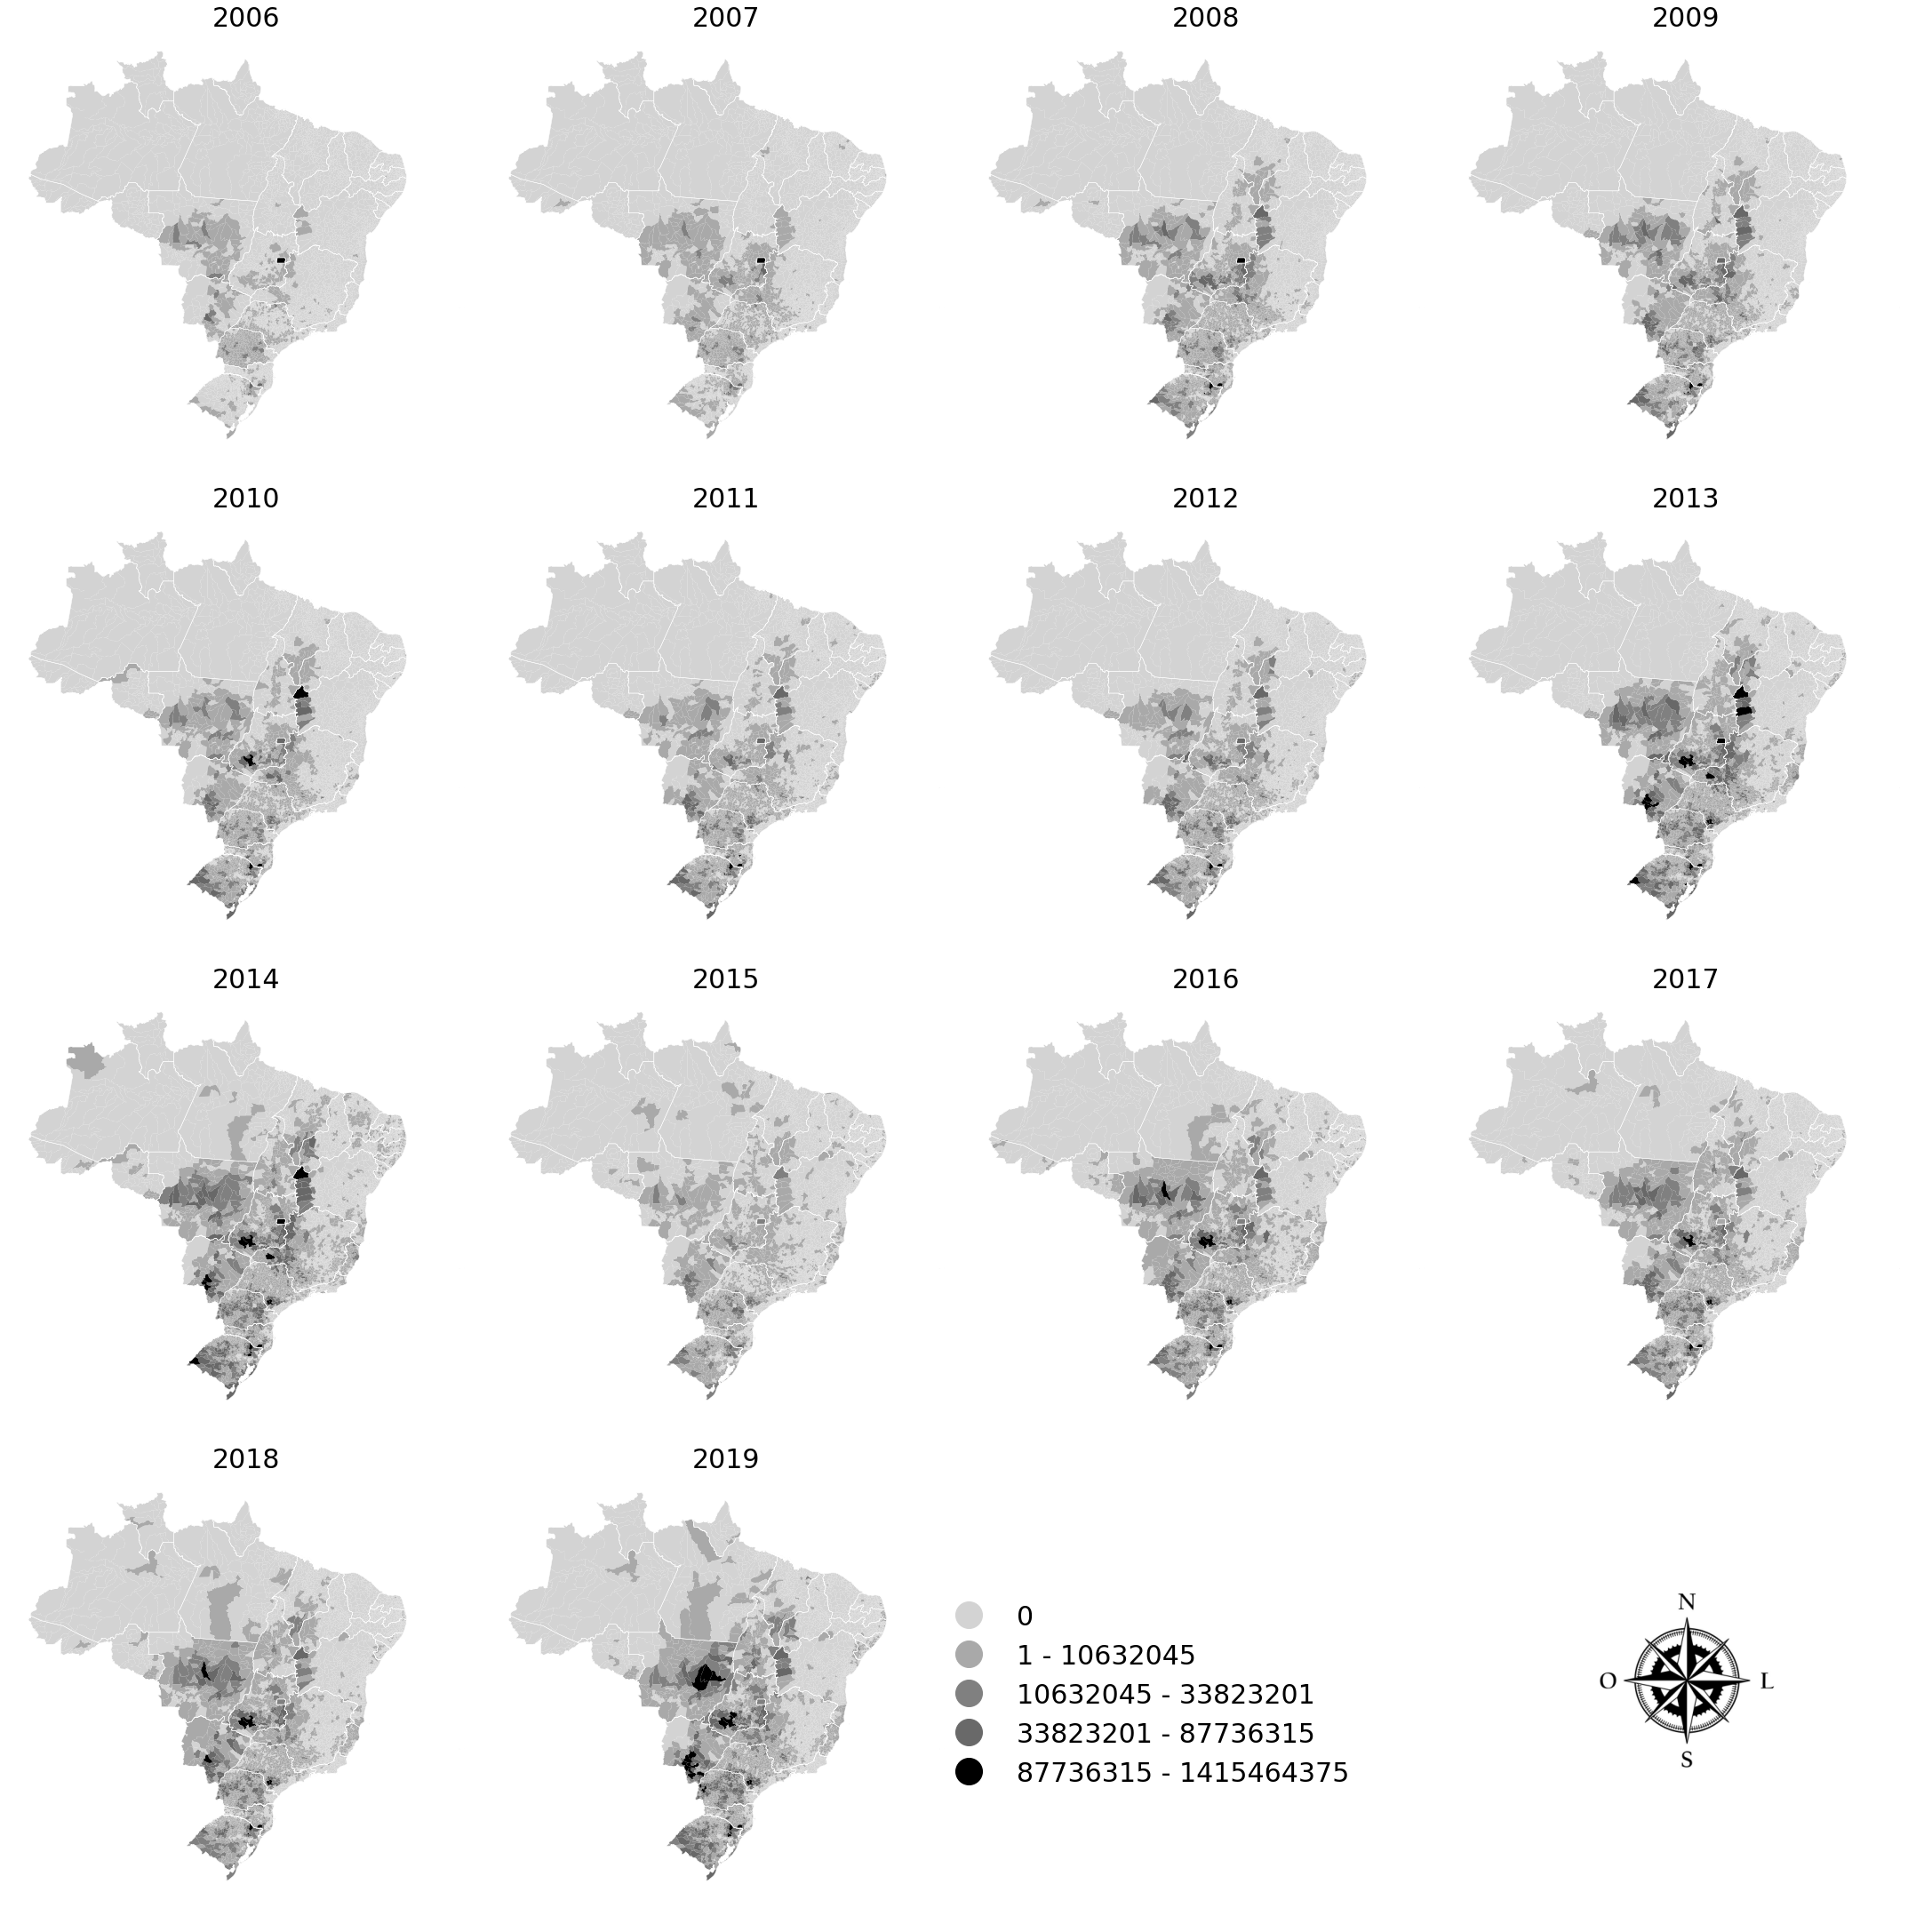
\includegraphics[width=0.9\textwidth]{figuras/map_total_segurado_mil.png}
	\small \textsuperscript {Fonte: Elaboração própria a partir de dados do Ministério da Agricultura, Pecuária e Abastecimento (MAPA)}
    \label{map_lisa_segurado}
\end{figure}

Pela análise da Figura \ref{map_apolices}, é possível observar que a distribuição espacial do número de apólices contratadas se modificou no decorrer dos anos, apesar de se concentrar principalmente nas Regiões Sul e Centro-Oeste. É possível também destacar que, durante o período analisado, há indícios de concentrações espaciais na região do Extremo Oeste Baiano no Estado da Bahia, Sudoeste de Mato Grosso do Sul, Sul Goiano no Estado de Goiás e Sudeste, no sul do Estado de São Paulo.

Ao longo dos anos, o número de municípios com nenhuma apólice contratada cai e há indícios de um aumento do número de apólices até o ano de $2014$. Entre os anos de $2014$ e $2015$,     há uma queda no número de apólices contratadas, como já foi mostrado no gráfico da Figura \ref{apolices_produtores}, e das demais variáveis relacionadas ao seguro rural. Essa redução também pode ser visualizada no mapa da Figura \ref{map_apolices}, em que o ano de $2015$ apresenta menos municípios com maior número de apólices contratadas. Ao se analisar a distribuição espacial, observa-se que há indícios de haver uma maior concentração espacial do número de apólices contratadas. A partir do ano de $2015$ a retomada do crescimento do número de apólices contratadas (Figura \ref{apolices_produtores}) pode ser visualizado com um maior número de áreas de coloração mais escura no mapa.

A distribuição espacial das demais variáveis analisadas apresenta um padrão semelhante ao observado com o número de apólices contratadas. Dessa forma, os resultados corroboram a hipótese apresentada por Silva, Teixeira e Santos (2014) na investigação sobre a participação do PSR na universalização do acesso ao seguro rural. Ou seja, apesar da evolução do seguro rural em âmbito nacional, quando se observa a distribuição espacial, verifica-se que há, ao longo do tempo, uma concentração das apólices e subvenções na região Sul. Portanto, apesar de ter ocorrido uma ampliação do seguro rural esta ampliação ocorreu de forma concentrada, o que evidencia o cumprimento de forma parcial dos objetivos do PSR \cite{silva14}.


\subsubsection{\textit{I} de Moran}

Uma vez feita a análise visual dos mapas temáticos, é necessário fazer uso de um teste estatístico para verificar se há evidências de padrões espaciais na distribuição dos dados. A estatística utilizada para esse fim foi o \textit{I} de Moran, sendo que para o seu cálculo foi adotada a matriz de vizinhança de continuidade binária do tipo rainha de primeira ordem. O pseudo valor-$p$ associado ao \textit{I} de Moran foi calculado a partir de 999 permutações aleatórias, conforme mencionado na seção \ref{material_e_metodos}.

O valor do \textit{I} de Moran foi calculado para cada variável e para todos os anos entre 2006 e 2019. Os resultados obtidos são apresentados na Tabela\ref{tab_moran} . Todos os valores do \textit{I} de Moran foram estatisticamente significativos ao nível de significância de $5\%$. 


\begin{small}
\begin{table}[H]
\caption{Autocorrelação espacial (\textit{I} de Moran) para as variáveis de seguro rural no Brasil por municípios entre 2006 e 2019} \label{tab_moran}
%\caption{I de Moran para as variáveis de seguro rural no Brasil por municípios entre 2006 e 2019} 
\footnotesize
\vspace{0.05cm}
%\label{moran_table}
\begin{tabularx}{\textwidth}{lXXXXXXXX}
    \hline \\[-1.9ex]	 
    Anos & ap\_contrat & t\_segurado & soma\_premio & t\_subvencao & inde\_pagas & sinis\_media & tx\_media & ap\_indeniz    \\
    \hline \\[-1.9ex]	 
    2006 & 0,562 & 0,002 & 0,161 &0,239 & 0,030 & 0,179 & 0,320 & 0,167 \\
    2007 & 0,496 & 0,146 & 0,183 &0,220 & 0,098 & 0,052 & 0,009 & 0,228 \\
    2008 & 0,471 & 0,303 & 0,298 &0,326 & 0,402 & 0,558 & 0,611 & 0,448 \\
    2009 & 0,503 & 0,390 & 0,340 &0,338 & 0,229 & 0,233 & 0,711 & 0,326 \\
    2010 & 0,477 & 0,345 & 0,292 &0,292 & 0,178 & 0,136 & 0,532 & 0,239 \\
    2011 & 0,510 & 0,388 & 0,318 &0,313 & 0,339 & 0,220 & 0,711 & 0,411 \\
    2012 & 0,542 & 0,443 & 0,377 &0,378 & 0,223 & 0,520 & 0,729 & 0,420 \\
    2013 & 0,563 & 0,413 & 0,424 &0,434 & 0,308 & 0,480 & 0,732 & 0,496 \\
    2014 & 0,590 & 0,434 & 0,409 &0,417 & 0,299 & 0,392 & 0,786 & 0,453 \\
    2015 & 0,601 & 0,458 & 0,408 &0,414 & 0,460 & 0,567 & 0,784 & 0,544 \\
    2016 & 0,589 & 0,473 & 0,396 &0,421 & 0,216 & 0,509 & 0,775 & 0,477 \\
    2017 & 0,607 & 0,482 & 0,391 &0,390 & 0,187 & 0,407 & 0,756 & 0,336 \\
    2018 & 0,617 & 0,487 & 0,418 &0,418 & 0,520 & 0,704 & 0,800 & 0,584 \\
    2019 & 0,636 & 0,520 & 0,506 &0,510 & 0,371 & 0,542 & 0,803 & 0,501 \\
	\hline 
\end{tabularx}
%\vspace{0.5cm}
\footnotesize{Fonte: Elaboração própria.  }\\
\footnotesize{Nota: Os valores do \textit{I} de Moran foram estatisticamente significativos em todas variáveis (valor$-p<0,005$)}\\
\end{table}
\end{small}

Todos os valores do \textit{I} de Moran foram positivos e significativos, o que indica que foi constatada uma autocorrelação espacial positiva entre os municípios brasileiros para as variáveis de seguro rural. Ou seja, o fato de um município possuir um maior número de apólices de seguro rural contratadas é influenciado, além de outros fatores, pelo número de apólices de seguro rural contratadas em sua região vizinha. Esse padrão de autocorrelação positiva também se aplica para as demais variáveis. Ou seja, o fato de um município possuir um valor da soma da importância segurada alta é influenciado, dentre outros fatores, pela soma da importância segurada nos municípios em seu entorno. O mesmo se aplica às variáveis soma dos prêmios, total da subvenção, soma das indenizações pagas, sinistralidade média, taxa média aplicada às apólices e número de apólices indenizadas. 

Além da presença de autocorrelação positiva em todos os anos, a análise da Tabela \ref{tab_moran} indica que a dependência espacial foi aumentando no decorrer dos anos em todas as variáveis. Ao analisar a autocorrelação espacial global da variável apólices contratadas, observa-se que, o menor valor da estatística foi  $0,471$ em $2008$, e o maior valor foi 0,636, em 2019. Também é possível observar que, há um crescimento do \textit{I} de Moram entre o ano de $2006$ e $2019$. Com relação ao número de apólices indenizadas nos municípios, constata-se que o menor valor da autocorrelação espacial global ocorreu em $2006$, e foi igual a $0,167$, sendo que o maior valor, por sua vez, foi de $0,584$ no ano de $2018$. %No período analisado, a autocorrelação espacial do número de apólices indenizadas nos municípios apresentou um aumento de cerca de 200\%.  

%Também é possível observar que há um crescimento de 11,64\% entre o ano de 2006 e 2019. Com relação ao número de apólices indenizadas nos municípios, constata-se que o menor valor da autocorrelação espacial global ocorreu em 2006 e foi igual a 0,167, o maior valor, por sua vez,  foi de 0,584 no ano de 2018. No período analisado, a autocorrelação espacial do número de apólices indenizadas nos municípios apresentou um aumento de cerca de 200\%.  

A autocorrelação espacial do total segurado apresentou um aumento de $25900\%$, sendo que o menor valor foi observado em $2006$ e o maior em $2019$, $0,002$ e $0,52$, respectivamente. A variável soma do prêmio total apresentou um aumento da autocorrelação espacial de cerca de $214\%$, com menor valor foi igual a $0,161$ em $2006$ e o valor máximo foi de $0,506$ em $2019$. Por sua vez, o total do valor subvencionado apresentou um aumento na autocorrelação espacial de $0,22$, em  $2007$, para $0,51$ em $2019$.

Para facilitar a visualização da evolução da autocorrelação espacial das variáveis, os valores do \textit{I} de Moran são apresentados do gráfico da Figura \ref{i_moran_anos}.

\begin{figure}[!htp]
	\centering
	\caption{Evolução dos valores de autocorrelação espacial (\textit{I} de Moran) entre os anos de $2006$ e $2019$}
	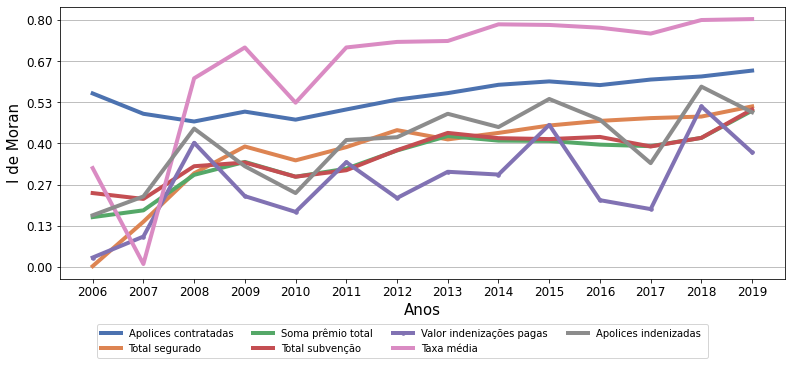
\includegraphics[width=0.8\textwidth]{figuras/i_de_moran.png}\\
	\small \textsuperscript {Fonte: Elaboração própria.}
    \label{i_moran_anos}
\end{figure}

É possível observar que, durante o período analisado, houve um aumento da autocorrelação espacial em todas as variáveis. Vale a pena destacar que, variáveis como apólices indenizadas, valor das indenizações pagas e sinistralidade média apresentaram maiores oscilações nos valores do \textit{I} de Moran. Esse comportamento pode ser devido, entre outras causas, à aleatoriedade da ocorrência de sinistros. 

% Ao analisar a correlação espacial de dados de produtividade das culturas de milho e soja no Estado do Paraná entre 1990 e 2002, Ozaki (2008) aponta que há um padrão de dependência espacial nos dados e, dessa forma, as unidades seguradas não podem ser consideradas espacialmente independentes. Além disso, Ozaki (2008) destaca que a presença de dependência espacial implica em sérias consequências no mercado de seguros agrícolas, pois o risco de insolvência das seguradoras frente aos segurados é grande, na ocorrência de um evento climático extremo. Nesse sentido, portanto, as seguradoras devem se atentar a estratégias que possibilitem uma diversificação geográfica e a concentração de riscos em determinadas regiões deve ser evitada.

\subsubsection{\textit{I} de Moran local}

O último passo da AEDE consistiu na construção dos mapas \textit{LISA}. Esses mapas apresentam $4$ grupos com características distintas de associação espacial estatisticamente significativas. 
Os mapas \textit{LISA} apresentados  na Figura \ref{map_lisa_contratadas}, apresentam os agrupamentos da variável apólices contratadas que foram estatisticamente significativos em cada um dos anos em análise. 

\begin{figure}[!htp]
	\centering
	\caption{Mapas \textit{LISA} para o número de apólices de seguro rural contratadas por municípios brasileiros, de 2006 a 2019}
	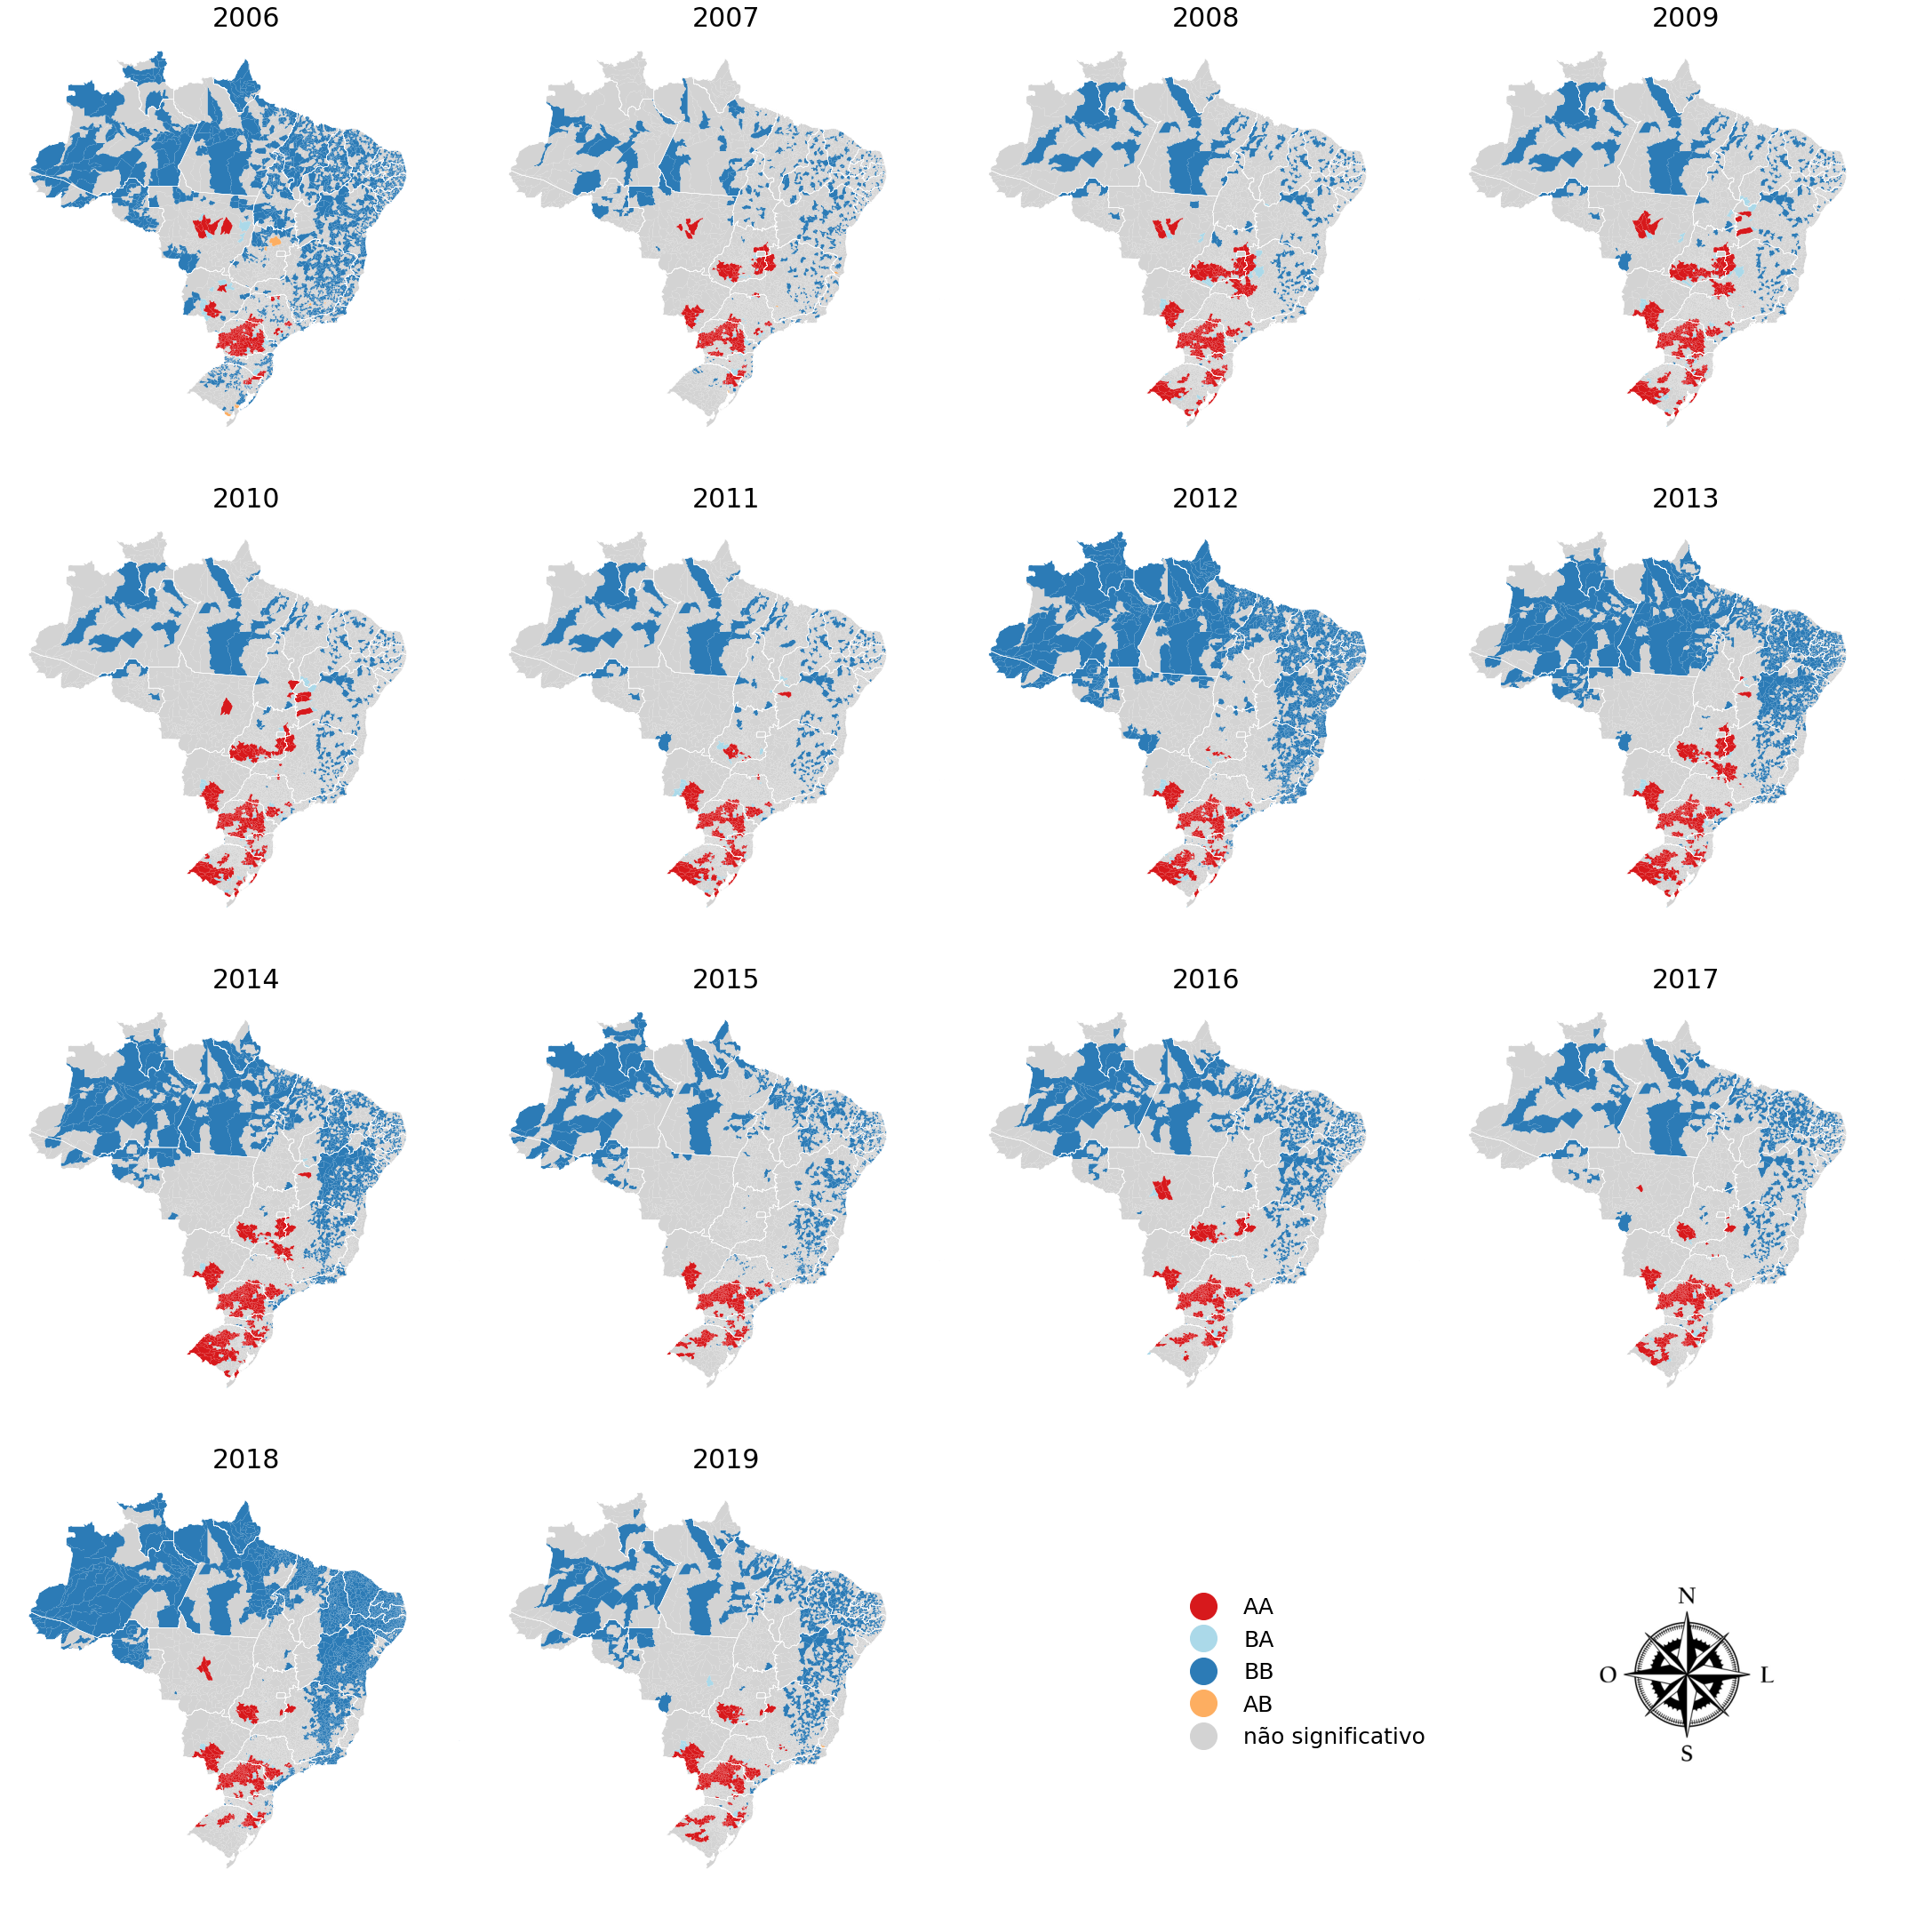
\includegraphics[width=0.9\textwidth]{figuras/map_lisa_apolices_contratadas.png}\\
	\small \textsuperscript {Fonte: Elaboração própria a partir de dados do Ministério da Agricultura, Pecuária e Abastecimento (MAPA)}
    \label{map_lisa_contratadas}
\end{figure}

No ano de $2006$, os agrupamentos do tipo AA, ou seja, agrupamentos formados por municípios com alta adesão a contratação de seguro rural que possuíam vizinhos também com alta adesão a esse tipo de seguro, estavam concentrados exclusivamente nas regiões Sudeste e Sul. Na região Sudeste, em $2006$, $32,3\%$ desses  municípios pertenciam ao estado de São Paulo e $3,08\%$ ao estado de Minas Gerais. Em $2006$, a região Sul possuía $64,62\%$ dos municípios do grupo AA, sendo que $24,62\%$ destes pertenciam ao estado do Rio Grande do Sul, $23,08\%$ ao Paraná e $16,92\%$ à Santa Catarina.  

Em $2019$, os agrupamentos do tipo AA são formados por municípios das regiões Centro-Oeste, Sudeste e Sul. A região Centro-Oeste contava, em $2019$, com $9,04\%$ dos municípios do grupo AA, a região Sudeste contava com $8,73\%$  e a região Sul com $82.23\%$. Na região Sul, $54,82\%$ pertenciam ao estado do Paraná, $25\%$ ao Rio Grande do Sul e $2,4\%$ a Santa Catarina. Essa distribuição dos municípios pertencentes ao grupo AA indica que, ao longo dos anos, apesar de mais regiões passarem a contar com municípios do grupo AA, houve uma concentração nos estados da região Sul, especialmente no estado do Paraná.

Segundo Santos e Silva (2017), historicamente, as apólices contratadas de seguro rural, o valor segurado e, por consequência, o valor de subvenção através do PSR se concentram regionalmente. Isto se dá devido à presença de maiores riscos de intempéries nos estados da Região Sul, em São Paulo e Minas Gerais. Estados como Mato Grosso do Sul, Mato Grosso, Goiás, e a região formada pelos estados do Maranhão, Tocantins, Piauí e Bahia, mais recentemente, também têm aderido aos contratos de seguro rural devido a fatores climáticos. 

Diversos fatores podem ser apontados como determinantes da concentração do mercado de seguro rural em poucas regiões, poucas culturas, com participação reduzida de seguradoras. Segundo Santos, Sousa e Alvarenga (2013), alguns fatores que devem ser considerados são: o pequeno número e a discrepância no porte das seguradoras que ofertam esse tipo de seguro, dificuldades das instituições bancárias com operações no meio rural, levando a informações imprecisas e à elevação de riscos e preços, parcerias governamentais com operadores, como por exemplo, programas de crédito oficial operados pelo Banco do Brasil, que também é o controlador da maior seguradora agrícola,  o grau de oportunidade avaliado como pequeno pelas seguradoras, e por fim, o pequeno peso de parcerias e de avaliação das oportunidades envolvendo o segmento de corretagem.   

%\newpage
\section{CONSIDERAÇÕES FINAIS}

O objetivo do presente trabalho foi analisar a evolução e a dinâmica espacial de variáveis do seguro rural nos municípios brasileiros entre 2006 e 2019. Além disso, buscou-se investigar a presença de padrões de distribuição espacial, por meio da autocorrelação espacial, bem como a existência de agrupamentos locais de distribuição espacial.

A análise possibilitou constatar resultados positivos na evolução do seguro rural no Brasil. O número de apólices contratadas tem um crescimento de cerca de $769,34\%$ durante o período. Ademais, a área agrícola segurada no país praticamente dobrou entre os anos de $2019$ e $2020$, quando alcançou o maior valor, $13,7$ milhões de hectares, que representa $20\%$ da área total agrícola do país. 

Os resultados da AEDE apontam que existe dependência espacial em todos os anos analisados. Ou seja, existem padrões de associação espacial estatisticamente significativos. Também foi possível identificar a presença de \textit{clusters} espaciais significativos. Tal resultado é observado em todas as variáveis de seguro rural analisadas. 

Em geral, identificou-se que as maiores concentrações de apólices de seguro rural estão situadas nas regiões Sul, Centro-Oeste e Sudeste, no sul do Estado de São Paulo. Além disso, foi constatado que há um aumento na dependência espacial do seguro rural ao longo do período analisado. Ou seja, municípios que possuem uma maior adesão ao seguro rural tendem a ser geograficamente próximos de municípios que também têm maior número de apólices de seguro rural contratadas. Para mais, ressalta-se que, embora mantenham a concentração do número de apólices contratadas, número de apólices indenizadas, valores de subvenção, indenização e prêmio, atualmente há expansão da demanda por seguros agrícolas. 

Apesar de os dados indicarem uma concentração geográfica da adesão ao sistema de seguro rural no Brasil, é necessário levar em consideração outros sistemas, como o Proagro e o programa Garantia Safra. É necessário, ainda, ressaltar que a adesão dos produtores deve ocorrer como uma resposta à percepção do risco das atividades agropecuárias, ou seja, o seguro deve difundir-se com base na compreensão dos riscos e das vantagens de sua contratação. 

Por fim, este trabalho pode ser entendido como uma abordagem inicial, a partir da qual é possível se introduzir novos métodos estatísticos a fim de aprimorar os resultados. Dentre esses métodos, destaca-se a Análise de Componentes Principais (ACP), que pode ser utilizada para reduzir o número de variáveis,  de forma a possibilitar a incorporação de informação de mais de uma variável na análise exploratória espacial.

\newpage
\addcontentsline{toc}{section}{\hspace*{\distnumber}REFERÊNCIAS}
\begin{center}
\section*{REFERÊNCIAS} 
\end{center}


